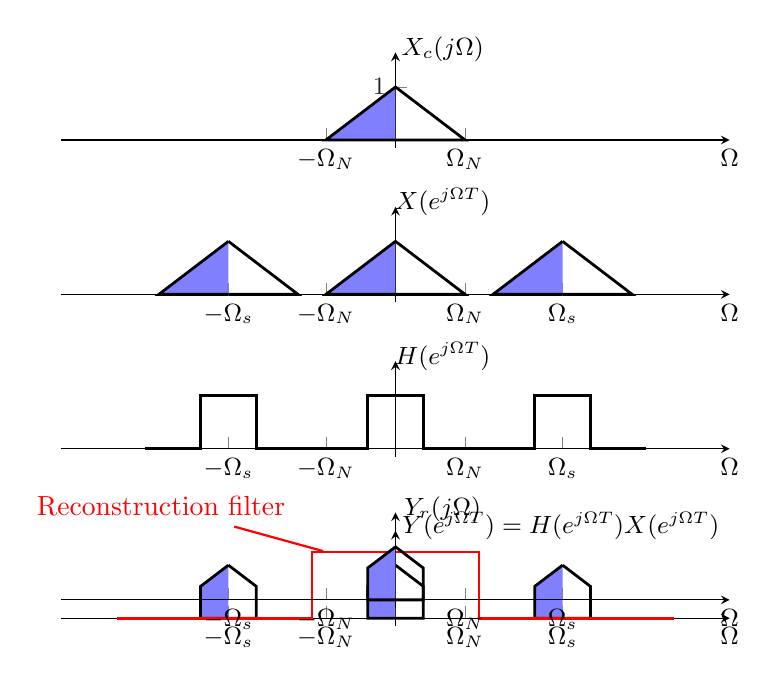
\begin{tikzpicture}
\onslide<1-|handout:1-2>{
	\begin{axis}[
	name=plot1,
	axis lines*=middle,
	enlargelimits = true,
	clip=false,
	scale only axis,
	width=0.7\textwidth,
	height=0.1\textwidth,
	ymin=0,
	ymax=3,
	xmin=-10,
	xmax=10,
	axis line style={->,>=stealth},
	xlabel={\small $\Omega$},
	ylabel={\small $X_c(j\Omega)$},
	every axis x label/.style={
		at={(ticklabel* cs:1)},
		%xshift=0.2cm,
		anchor=north,
	},
	every axis y label/.style={
		at={(ticklabel* cs:0.8)},
		anchor=south,
		xshift=0.6cm,
	},
	ytick=2,
	xtick=\empty,
	yticklabel={\small 1},
	xtick={-2.5, 2.5},
	xticklabels={\small $-\Omega_N$, \small $\Omega_N$},
	every outer y axis line/.append style={white!15!black},
	every y tick label/.append style={font=\color{white!15!black}},
	legend style={draw=white!15!black,fill=white,legend cell align=left}]
	\addplot[solid, line width=1pt] coordinates {(0, 2) (2.5, 0) (0, 0)};
	\addplot[solid, line width=1pt, fill=blue!50] coordinates {(0, 2) (-2.5, 0) (0, 0)};
	\end{axis}
}
\onslide<2-|handout:1-2>{
	\begin{axis}[
	name=plot2,
	at=(plot1.below south east), anchor=above north east,
	axis lines*=middle,
	enlargelimits = true,
	clip=false,
	scale only axis,
	width=0.7\textwidth,
	height=0.1\textwidth,
	ymin=0,
	ymax=3,
	xmin=-10,
	xmax=10,
	axis line style={->,>=stealth},
	xlabel={\small $\Omega$},
	ylabel={\small $X(e^{j\Omega T})$},
	yticklabel style = {yshift=0.1cm},
	every axis x label/.style={
		at={(ticklabel* cs:1)},
		%xshift=0.2cm,
		anchor=north,
	},
	every axis y label/.style={
		at={(ticklabel* cs:0.8)},
		anchor=south,
		xshift=0.6cm,
	},
	ytick=\empty,
	xtick={-6, -2.5, 0, 2.5, 6},
	xticklabels={\small $-\Omega_s$, \small $-\Omega_N$, \small 0, \small $\Omega_N$, \small $\Omega_s$}, 
	every outer y axis line/.append style={white!15!black},
	every y tick label/.append style={font=\color{white!15!black}},
	legend style={draw=white!15!black,fill=white,legend cell align=left}]
	\addplot[solid, line width=1pt] coordinates {(0, 2) (2.5, 0) (0, 0)};
	\addplot[solid, line width=1pt, fill=blue!50] coordinates {(0, 2) (-2.5, 0) (0, 0)};
	\addplot[solid, line width=1pt] coordinates {(6, 2) (8.5, 0) (6, 0)};
	\addplot[solid, line width=1pt, fill=blue!50] coordinates {(6, 2) (3.5, 0) (6, 0)};
	\addplot[solid, line width=1pt] coordinates {(-6, 2) (-3.5, 0) (-6, 0)};
	\addplot[solid, line width=1pt, fill=blue!50] coordinates {(-6, 2) (-8.5, 0) (-6, 0)};
	\end{axis}
}
\onslide<3-|handout:1-2>{
	\begin{axis}[
	name=plot3,
	at=(plot2.below south east), anchor=above north east,
	axis lines*=middle,
	enlargelimits = true,
	clip=false,
	scale only axis,
	width=0.7\textwidth,
	height=0.1\textwidth,
	ymin=0,
	ymax=3,
	xmin=-10,
	xmax=10,
	axis line style={->,>=stealth},
	xlabel={\small $\Omega$},
	ylabel={\small $H(e^{j\Omega T})$},
	every axis x label/.style={
		at={(ticklabel* cs:1)},
		%xshift=0.2cm,
		anchor=north,
	},
	every axis y label/.style={
		at={(ticklabel* cs:0.8)},
		anchor=south,
		xshift=0.6cm,
	},
	xtick=\empty,
	ytick=\empty,
	xtick={-6, -2.5, 0, 2.5, 6},
	xticklabels={\small $-\Omega_s$, \small $-\Omega_N$, \small 0, \small $\Omega_N$, \small $\Omega_s$}, 
	every outer y axis line/.append style={white!15!black},
	every y tick label/.append style={font=\color{white!15!black}},
	legend style={draw=white!15!black,fill=white,legend cell align=left}]
	\addplot[solid, line width=1pt] coordinates {(-3, 0) (-1, 0) (-1, 2) (1, 2) (1, 0) (3, 0)};
	\addplot[solid, line width=1pt] coordinates {(-9, 0) (-7, 0) (-7, 2) (-5, 2) (-5, 0) (-3, 0)};
	\addplot[solid, line width=1pt] coordinates {(3, 0) (5, 0) (5, 2) (7, 2) (7, 0) (9, 0)};	
	\end{axis}
}

\onslide<4-5|handout:1>{
	\begin{axis}[
	name=plot4,
	at=(plot3.below south east), anchor=above north east,
	axis lines*=middle,
	enlargelimits = true,
	clip=false,
	scale only axis,
	width=0.7\textwidth,
	height=0.1\textwidth,
	ymin=0,
	ymax=3,
	xmin=-10,
	xmax=10,
	axis line style={->,>=stealth},
	xlabel={\small $\Omega$},
	ylabel={\small $Y(e^{j\Omega T}) = H(e^{j\Omega T})X(e^{j\Omega T})$},
	every axis x label/.style={
		at={(ticklabel* cs:1)},
		%xshift=0.2cm,
		anchor=north,
	},
	every axis y label/.style={
		at={(ticklabel* cs:0.8)},
		anchor=south,
		xshift=2.1cm,
	},
	xtick=\empty,
	ytick=\empty,
	xtick={-6, -2.5, 0, 2.5, 6},
	xticklabels={\small $-\Omega_s$, \small $-\Omega_N$, \small 0, \small $\Omega_N$, \small $\Omega_s$}, 
	every outer y axis line/.append style={white!15!black},
	every y tick label/.append style={font=\color{white!15!black}},
	legend style={draw=white!15!black,fill=white,legend cell align=left}]
	\addplot[solid, line width=1pt, fill=blue!50] coordinates {(0, 0) (-1, 0) (-1, 1.2) (0, 2)}; 
	\addplot[solid, line width=1pt] coordinates {(0, 0) (1, 0) (1, 1.2) (0, 2)};
	\addplot[solid, line width=1pt, fill=blue!50] coordinates {(-6, 0) (-7, 0) (-7, 1.2) (-6, 2)}; 
	\addplot[solid, line width=1pt] coordinates {(-6, 0) (-5, 0) (-5, 1.2) (-6, 2)};
	\addplot[solid, line width=1pt, fill=blue!50] coordinates {(6, 0) (5, 0) (5, 1.2) (6, 2)}; 
	\addplot[solid, line width=1pt] coordinates {(6, 0) (7, 0) (7, 1.2) (6, 2)};
	
	\only<5|handout:1>{
		\addplot[red, solid, line width=1pt] coordinates {(-10, 0) (-3, 0) (-3, 2.5) (3, 2.5) (3, 0) (10, 0)} node[pos=0.4, red, pin={[pin edge={red, thick}]140:{Reconstruction filter}}, inner sep=0pt] {};
	}
	\end{axis}
}

\onslide<6|handout:2>{
	\begin{axis}[
	name=plot4,
	at=(plot3.below south east), anchor=above north east,
	axis lines*=middle,
	enlargelimits = true,
	clip=false,
	scale only axis,
	width=0.7\textwidth,
	height=0.1\textwidth,
	ymin=0,
	ymax=3,
	xmin=-10,
	xmax=10,
	axis line style={->,>=stealth},
	xlabel={\small $\Omega$},
	ylabel={\small $Y_r(j\Omega)$},
	every axis x label/.style={
		at={(ticklabel* cs:1)},
		%xshift=0.2cm,
		anchor=north,
	},
	every axis y label/.style={
		at={(ticklabel* cs:0.8)},
		anchor=south,
		xshift=0.6cm,
	},
	xtick=\empty,
	ytick=\empty,
	xtick={-6, -2.5, 0, 2.5, 6},
	xticklabels={\small $-\Omega_s$, \small $-\Omega_N$, \small 0, \small $\Omega_N$, \small $\Omega_s$}, 
	every outer y axis line/.append style={white!15!black},
	every y tick label/.append style={font=\color{white!15!black}},
	legend style={draw=white!15!black,fill=white,legend cell align=left}]
	\addplot[solid, line width=1pt, fill=blue!50] coordinates {(0, 0) (-1, 0) (-1, 1.2) (0, 2)}; 
	\addplot[solid, line width=1pt] coordinates {(0, 0) (1, 0) (1, 1.2) (0, 2)};
	\end{axis}
}
\end{tikzpicture}
